\documentclass[a4paper,10pt]{article}
\usepackage{lamia-pedagogy}

\begin{document}

% =========================================================================
% PAGE 1 : Fiche Enseignant & Texte Support
% =========================================================================
\ficheHeader{1 Heure}{\makebox[2.5cm]{\dotfill}}{1\textsuperscript{ère} AM}{2026 / 2027}

\vspace{-3pt}
\competenceBanner{\faBookReader\ Projet 01 / Séquence 01 — Séance 07 : Compréhension de l'Écrit (02)}

\vspace{-2pt}
\modaliteSupportBar{Lecture individuelle puis collective}{Manuel scolaire p. 26 / Support : \guillemotleft\ Les caries dentaires \guillemotright}

\vspace{1pt}

% Texte support
\begin{tcolorbox}[
  enhanced,
  colback=primarylight!40,
  colframe=primary,
  arc=2mm,boxrule=0.8pt,
  top=5pt,bottom=5pt,left=8pt,right=8pt,
  title={\small\textbf{\textcolor{white}{\faFileMedical\ Texte : Les caries dentaires (Manuel p. 26)}}},
  coltitle=white,colbacktitle=primary
]
{\small
La carie dentaire peut évoluer pendant plusieurs semaines sans provoquer de douleur. Mais qu'est-ce qui la provoque ?

\textbf{La carie dentaire est une infection des tissus de la dent.} Elle est souvent provoquée par les aliments sucrés que les enfants consomment en grande quantité sans se brosser les dents ou pas régulièrement. Lorsqu'ils le font, ils n'utilisent pas un dentifrice au fluor. Or, chaque brossage doit durer au moins trois minutes pour être efficace.

Comme on le voit, les caries dentaires sont un problème de santé bucco-dentaire grave. Il doit être combattu très sérieusement par une hygiène quotidienne et des visites régulières chez le dentiste.

\hfill\textit{\footnotesize D'après les guides de santé scolaire}
}
\end{tcolorbox}

\vspace{3pt}

% Tableau de Structuration
\begin{tcolorbox}[
  enhanced,
  colback=white,
  colframe=cardborder,
  arc=2mm,boxrule=0.7pt,
  top=4pt,bottom=4pt,left=7pt,right=7pt,
  title={\small\textbf{\textcolor{primary}{\faTable\ Tableau de structuration du texte explicatif}}},
  coltitle=primary,colbacktitle=primarylight,titlerule=0.4pt
]
{\footnotesize
\begin{tabularx}{\linewidth}{|l|X|X|}
\hline
\rowcolor{primarylight}\textbf{Phases du texte} & \textbf{Parties du texte} & \textbf{Contenu explicatif} \\
\hline
\textbf{1. Questionnement} & 1\textsuperscript{er} paragraphe & Constat et interrogation de départ (\textit{Qu'est-ce qui la provoque ?}). \\
\hline
\textbf{2. Explication} & 2\textsuperscript{ème} paragraphe & Définition de la carie, causes (sucreries, manque d'hygiène) et durée du brossage. \\
\hline
\textbf{3. Conclusion} & 3\textsuperscript{ème} paragraphe & Bilan et recommandation (consulter le dentiste, brossage quotidien). \\
\hline
\end{tabularx}
}
\end{tcolorbox}

\vspace{3pt}

% Objectifs
\begin{tcolorbox}[
  enhanced,
  colback=secondarylight!50,
  colframe=secondary,
  arc=1.5mm,leftrule=3pt,rightrule=0.5pt,toprule=0.5pt,bottomrule=0.5pt,
  top=3pt,bottom=3pt,left=6pt,right=6pt
]
{\footnotesize
\textbf{\faBullseye\ Objectifs d'apprentissage :} Identifier la structure tripartite du texte explicatif, repérer une définition et des relations de cause à effet relatives à l'hygiène bucco-dentaire.
}
\end{tcolorbox}

\newpage

% =========================================================================
% PAGE 2 : Fiche d'Exploitation Élève & Support Illustré
% =========================================================================
\ficheHeader{1 Heure}{Nom : \makebox[4cm]{\dotfill}}{1\textsuperscript{ère} AM}{Classe : \makebox[1.5cm]{\dotfill}}

\vspace{-3pt}
\competenceBanner{\faPenFancy\ Questionnaire d'Analyse : Les Caries Dentaires}

\vspace{2pt}

\begin{minipage}[t]{0.62\textwidth}
% ACTIVITÉ 1 : Étude de texte
\begin{tcolorbox}[
  enhanced,
  colback=white,
  colframe=cardborder,
  arc=2mm,boxrule=0.8pt,
  top=4pt,bottom=4pt,left=7pt,right=7pt,
  title={\small\textbf{\textcolor{primary}{\faCheckSquare\ Activité 01 : Exploitation du texte}} \hfill \badge[primary]{Compréhension}},
  coltitle=primary,colbacktitle=primarylight,titlerule=0.5pt,titlerule style=cardborder
]
{\small
\begin{enumerate}[label=\textbf{\arabic*.},leftmargin=*,noitemsep,topsep=2pt]
  \item Quel est le type de ce texte ?
    \cardOptTwo{Narratif (qui raconte)}{Explicatif (qui explique)}
  \item Relève dans le texte la définition de la carie :\\
    \drule{\linewidth}\\[4pt]
    \drule{\linewidth}
  \item Quelles sont les principales causes de la carie ?
    \begin{itemize}[leftmargin=*,noitemsep,topsep=1pt]
      \item \drule{6.2cm}
      \item \drule{6.2cm}
    \end{itemize}
  \item Combien de temps doit durer chaque brossage ?
    \cardOptThree{1 minute}{3 minutes}{10 minutes}
\end{enumerate}
}
\end{tcolorbox}
\end{minipage}%
\hfill
\begin{minipage}[t]{0.36\textwidth}
% Illustration Support
\begin{tcolorbox}[
  enhanced,
  colback=white,
  colframe=cardborder,
  arc=2mm,boxrule=0.7pt,
  top=3pt,bottom=3pt,left=3pt,right=3pt,
  title={\scriptsize\textbf{\faTooth\ Schéma bucco-dentaire}},
  coltitle=primary,colbacktitle=primarylight,titlerule=0.4pt
]
\centering
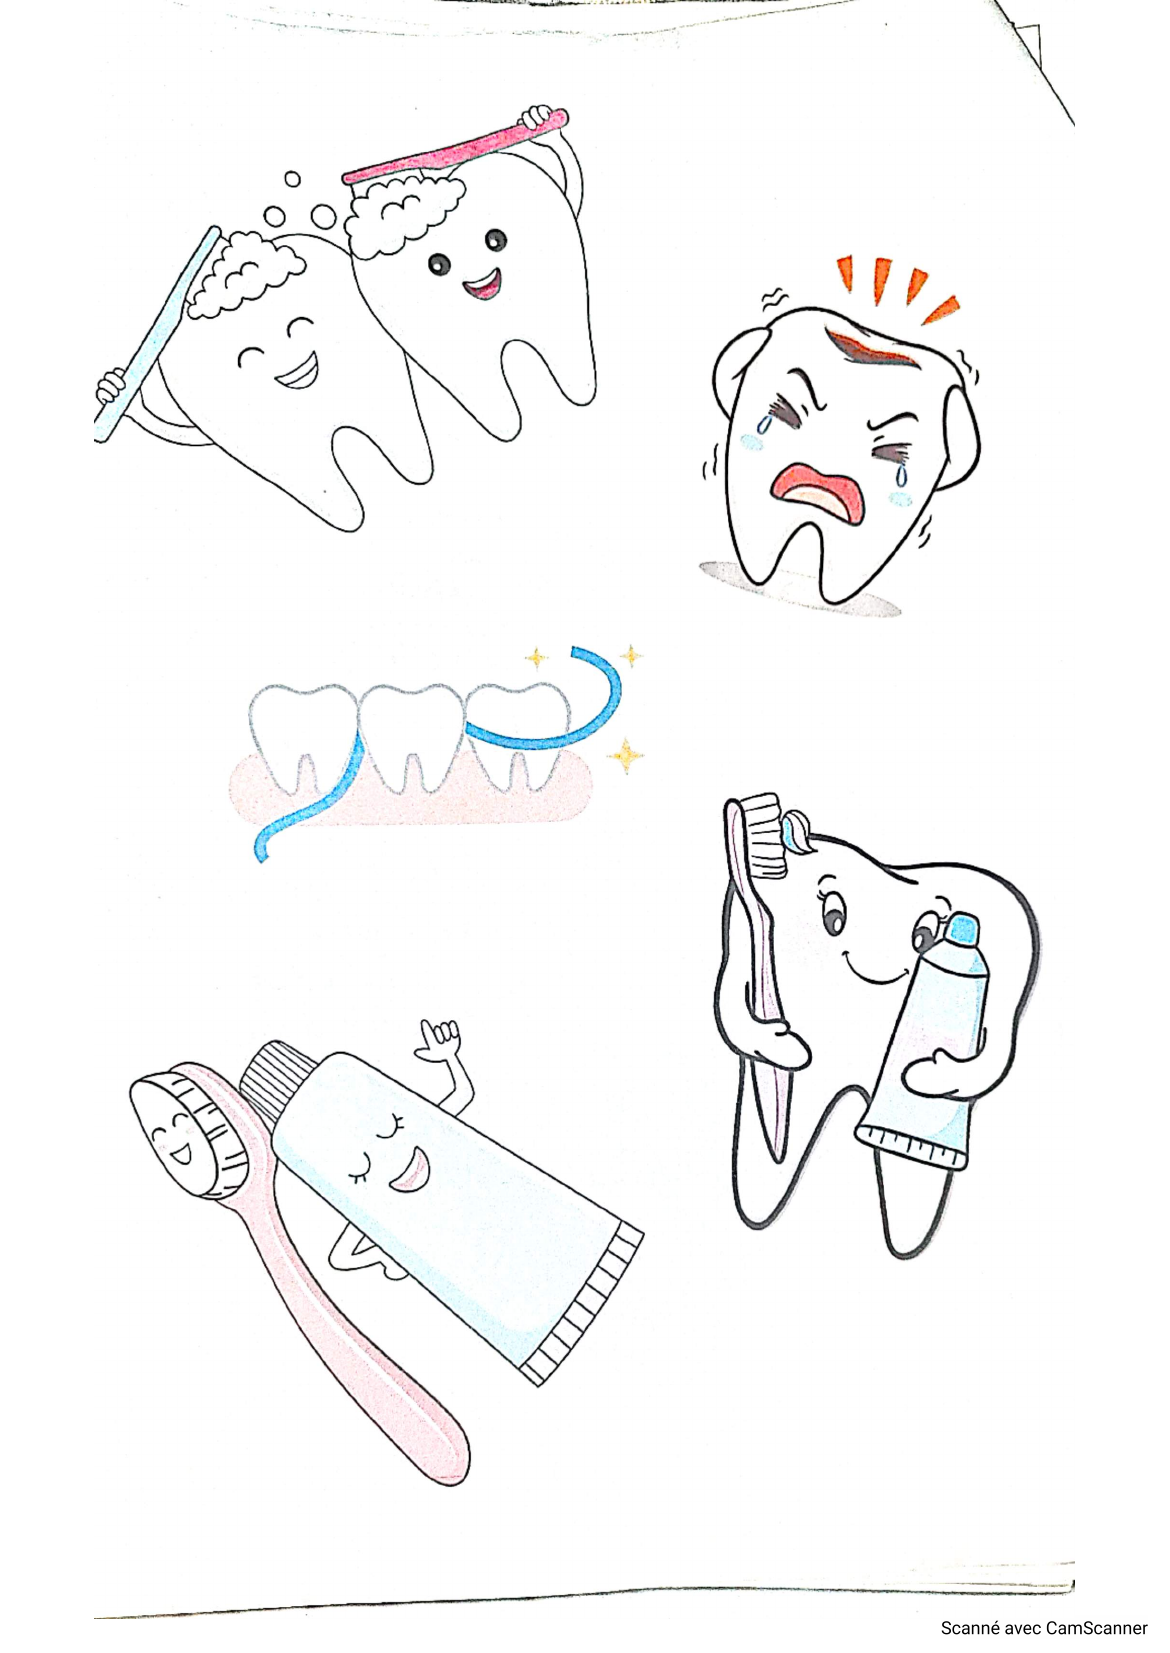
\includegraphics[width=\linewidth,height=7.2cm,keepaspectratio]{assets/images/caries_dents.png}
\end{tcolorbox}
\end{minipage}

\vspace{2pt}

% ACTIVITÉ 2 : Vrai ou Faux
\begin{tcolorbox}[
  enhanced,
  colback=white,
  colframe=cardborder,
  arc=2mm,boxrule=0.8pt,
  top=4pt,bottom=4pt,left=8pt,right=8pt,
  title={\small\textbf{\textcolor{primary}{\faCheckDouble\ Activité 02 : Réponds par Vrai ou Faux}} \hfill \badge[secondary]{Validation}},
  coltitle=primary,colbacktitle=primarylight,titlerule=0.5pt,titlerule style=cardborder
]
{\small
\begin{enumerate}[label=\textbf{\alph*)},leftmargin=*,noitemsep,topsep=2pt]
  \item La carie provoque immédiatement une douleur très vive. \dotfill \cardOptTwo{Vrai}{Faux}
  \item Le fluor aide à protéger et fortifier l'émail des dents. \dotfill \cardOptTwo{Vrai}{Faux}
  \item Manger beaucoup de sucreries favorise l'apparition des caries. \dotfill \cardOptTwo{Vrai}{Faux}
\end{enumerate}
}
\end{tcolorbox}

\vspace{2pt}

% ACTIVITÉ 3 : Synthèse
\begin{tcolorbox}[
  enhanced,
  colback=neutrallight,
  colframe=secondary!60!cardborder,
  arc=1.5mm,boxrule=0.6pt,
  top=3pt,bottom=3pt,left=7pt,right=7pt,
  title={\scriptsize\textbf{\faLightbulb\ Je retiens pour ma santé}},
  coltitle=primary,colbacktitle=secondarylight,titlerule=0.4pt
]
{\footnotesize
Pour garder des dents saines, je dois me brosser les dents \textbf{3 fois par jour} pendant \textbf{3 minutes} avec un dentifrice au fluor, et limiter la consommation de bonbons et de sodas.
}
\end{tcolorbox}

\end{document}
